\chapter{Prioritising COVID-19 vaccination in changing social and epidemiological landscapes: a mathematical modelling study}
\label{covidmodel}
\let\thefootnote\relax\footnote{This chapter is based on the paper: Jentsch, Peter C., Madhur Anand, and Chris T. Bauch. "Prioritising COVID-19 vaccination in changing social and epidemiological landscapes: a mathematical modelling study." The Lancet Infectious Diseases (2021).}
\begin{abstract}
  During the COVID-19 pandemic, authorities must decide which groups to prioritise for vaccination in a shifting social–epidemiological landscape in which the success of large-scale non-pharmaceutical interventions requires broad social acceptance. We aimed to compare projected COVID-19 mortality under four different strategies for the prioritisation of SARS-CoV-2 vaccines. We developed a coupled social–epidemiological model of SARS-CoV-2 transmission in which social and epidemiological dynamics interact with one another. We modelled how population adherence to non-pharmaceutical interventions responds to case incidence. In the model, schools and workplaces are also closed and reopened on the basis of reported cases. The model was parameterised with data on COVID-19 cases and mortality, SARS-CoV-2 seroprevalence, population mobility, and demography from Ontario, Canada (population 14.5 million). Disease progression parameters came from the SARS-CoV-2 epidemiological literature. We assumed a vaccine with 75\% efficacy against disease and transmissibility. We compared vaccinating those aged 60 years and older first (oldest-first strategy), vaccinating those younger than 20 years first (youngest-first strategy), vaccinating uniformly by age (uniform strategy), and a novel contact-based strategy. The latter three strategies interrupt transmission, whereas the first targets a vulnerable group to reduce disease. Vaccination rates ranged from 0.5\% to 5\% of the population per week, beginning on either Jan 1 or Sept 1, 2021. Case notifications, non-pharmaceutical intervention adherence, and lockdown undergo successive waves that interact with the timing of the vaccine programme to determine the relative effectiveness of the four strategies. Transmission-interrupting strategies become relatively more effective with time as herd immunity builds. The model predicts that, in the absence of vaccination, 72000 deaths (95\% credible interval 40000–122000) would occur in Ontario from Jan 1, 2021, to March 14, 2025, and at a vaccination rate of 1.5\% of the population per week, the oldest-first strategy would reduce COVID-19 mortality by 90.8\% on average (followed by 89.5\% in the uniform, 88.9\% in the contact-based, and 88.2\% in the youngest-first strategies). 60000 deaths (31000–108000) would occur from Sept 1, 2021, to March 14, 2025, in the absence of vaccination, and the contact-based strategy would reduce COVID-19 mortality by 92.6\% on average (followed by 92.1\% in the uniform, 91.0\% in the oldest-first, and 88.3\% in the youngest-first strategies) at a vaccination rate of 1.5\% of the population per week.Interpretation The most effective vaccination strategy for reducing mortality due to COVID-19 depends on the time course of the pandemic in the population. For later vaccination start dates, use of SARS-CoV-2 vaccines to interrupt transmission might prevent more deaths than prioritising vulnerable age groups.

\end{abstract}


\section{Introduction}


The COVID-19 pandemic has imposed a massive global health burden as waves of infection to move through populations around the world \cite{miller2020disease}.  Both empirical analyses and mathematical models conclude that non-pharmaceutical interventions (NPIs) are effective in reducing COVID-19 case incidence \cite{anderson2020estimating,peak2020individual,tuite2020mathematical}.  However, pharmaceutical interventions are highly desirable given the socio-economic costs of lockdown and physical distancing.  Hence, dozens of vaccines are  in development \cite{lurie2020developing}, and  model-based analyses are exploring the question of which groups should get the COVID-19 vaccine first \cite{bubar2020model,hoyt2020vaccine}.  


When vaccines become available, we will face a very different epidemiological landscape from the early pandemic. Many populations will already have experienced one or more waves of COVID-19.  As a result of natural immunity, the effective reproduction number $R_{eff}$ (the average number of secondary infections produced per infected person) will be reduced from its original value of approximately $R_0 = 2.2$ in the absence of pre-existing immunity \cite{hilton2020estimation}. Epidemiological theory tells us that as $R$ (or $R_0$) decline toward 1, the indirect benefits of transmission-blocking vaccines become stronger.  For instance, if $R_{eff} \approx 1.5$, such as for seasonal influenza, only an estimated $33 \%$ percent of the population needs immunity for transmission to die out in a homogeneously mixing population  \cite{anderson1992infectious,dushoff2007vaccinating}.  This effect was evidenced by the strong suppression of influenza incidence in Australia in Spring 2020 due to NPIs targeted against COVID-19 \cite{aussie2020}. 

This effect has stimulated a literature comparing the vaccination of groups that are responsible for most transmission to vaccination of groups that are vulnerable to serious complications from the infection. Natural immunity to SARS-CoV-2 will likely continue to rise in many populations on account of further infection waves. Given these likely changes to the epidemiological landscape before the vaccine becomes available, we suggest this question is worthy of investigation in the context of COVID-19. 


The social landscape will also look very different when vaccines become available and this aspect is crucial to understanding the pandemic. Scalable non-pharmaceutical interventions (NPIs) like physical distancing, hand-washing and masks are often one of the few available interventions when a novel pathogen emerges. Flattening the COVID-19 epidemic curve was possible due to a sufficient response by populations willing to adhere to public health recommendations. Therefore, pandemic waves are not simply imposed on populations -- they are a creation of the population response to the pathogen. They exemplify coupled socio-epidemiological systems exhibiting two-way feedback between disease dynamics and behavioural dynamics interact with one another \cite{pedro2020conditions}.

Approaches to modelling coupled social-epidemiological dynamics vary\cite{reluga2010game,salathe2008effect,funk2009spread,verelst2016behavioural,funk2010modelling}.  Some models have used evolutionary game theory to model this two-way feedback in a variety of coupled human-environment systems \cite{pedro2020conditions,bauch2005imitation,innes2013impact,bury2019charting,amaral2020epidemiological,zhao2020imitation,alam2020based}.  Evolutionary game theory captures how individuals learn social behaviours from others while weighing risks and benefits of different choices. In this framework, individuals who do not adopt NPIs can “free-ride” on the benefits of reduced transmission generated by individuals who do adopt NPIs \cite{reluga2010game}. 

Here, our objective is to compare projected COVID-19 mortality under four strategies for the prioritisation of COVID-19 vaccines: older individuals first, children first, uniform allocation, and a novel strategy based on the contact structure of the population. We use an age-structured model of SARS-CoV-2 transmission, including evolutionary game theory to model population adherence to NPIs and changes to mobility patterns.  We use scenario and sensitivity analysis to identify how strategy effectiveness responds to possible changes in the social-epidemiological landscape that may occur before and after vaccines become available.  

\section{Model Overview}

\subsection{Structure and parameterisation}

We developed an age-structured SEPAIR model (Susceptible, Exposed, Presymptomatic, Asymptomatic, Symptomatic, Removed) with ages in 5-year increments. Upon infection, individuals enter a latent period where they are infected but not yet infectious (“Exposed”).  After the latent period, individuals become presymptomatically infectious, and then either symptomatically or asymptomatically infectious, before finally entering the Removed compartment when their infectiousness ends. We did not model testing or contact tracing explicitly, although we assume infected individuals are ascertained at some rate. Transmission occurs through an age-specific contact matrix, susceptibility to infection is age-specific, and we include seasonality due to changes in the contact patterns throughout the year.  To infer model parameters, we fitted the model to Ontario COVID-19 case notifications stratified by age and time, Ontario seroprevalence data, and Ontario mobility data.  Use of seroprevalence data ensured that our estimates of transmission were not biased by case under-reporting. Remaining model parameter values were fixed using Ontario demographic and mortality data, and literature on COVID-19 serial interval and incubation periods. The system of differential equations comprising our model is solved numerically with DifferentialEquations.jl in the Julia language \cite{rackauckas2017differentialequations}.

Both schools and workplaces are closed when the number of ascertained active cases surpasses 50\%, 100\%, 150\%, 200\%, or 250\% of the peak ascertained active cases that occurred during the first wave (the “shutdown threshold”, T), and are re-opened again when cases fall below that threshold. Individuals interact with other individuals at a specified rate and switch between adherence and non-adherence to NPIs, including mobility restrictions, by comparing the cost of practicing NPIs against the cost of not practicing NPIs and thereby being subject to an increased risk of infection according to the prevalence of ascertained cases.  Both school and workplace closure and population level of adherence to NPIs reduce transmission according to a specified efficacy. 



\subsection{Model Equations}
 
Transmission dynamics are given by an SEPAIR model, modified to take population adherence to NPIs and school/workplace closure into account, and divided into age classes $i \in [1,16]$, where each age class contains a 5 year cohort, except for the oldest age group which comprises the ages $75$ and over. The model equations are:

\textcolor{black}{\begin{eqnarray}
\frac{dS^1_i}{dt} &= & S^1_i \left(- r \rho_i  \xi(t) \sum_{j=1}^{16} C_{ij}(t) \left(\frac{I_{s_j} + I_{a_j} + P_j}{N_j}\right) - \tau\right) \label{S1eqn} \\
\frac{dS^2_i}{dt} &= & S^2_i \left(- r \rho_i  \xi(t) \sum_{j=1}^{16} C_{ij}(t) \left(\frac{I_{s_j} + I_{a_j}+ P_j}{N_j}\right)  - \tau \right)  \label{S2eqn} \\
\frac{dE_i}{dt} &= &  (S^1_i + S^2_i) \left(r_i  \xi(t) \sum_{j=1}^{16} C_{ij}(t) \left(\frac{I_{s_j} + I_{a_j}+ P_j}{N_j}\right) - \sigma_0 E_i + \tau \right) \label{Eeqn} \\
\frac{dP_i}{dt} &= & \sigma_0 E_i - \sigma_1 P_i \label{Peqn} \\
\frac{dI_{a_i}}{dt} &= & \eta \sigma_1 E_i - \gamma_a I_{a_i}\label{Ieqn} \\
\frac{dI_{s_i}}{dt} &= & (1 - \eta) \sigma_1 E_i - \gamma_s I_{s_i} \label{Ieqn} \\
\frac{dR_i}{dt} &= & \gamma_a I_{a_i} + \gamma_s I_{s_i}  \label{Reqn} \\
\frac{dD_i}{dt} &= & \Omega(D(t)) \label{Deqn}
\end{eqnarray}}

where $\xi(t) = \left[1 + s \sin\left(\frac{2 \pi}{365} (t - \phi) - \frac{\pi}{2}\right)\right]$ determines the seasonally varying transmission rate with phase $\phi$ and amplitute $s$.

\noindent Parameter values are defined in Table \ref{tab:params}. The vaccination dynamics are an impulsive process applied each day, described below. $S^{1}_i$ is the number of unvaccinated susceptible individuals in age group $i$, and $S^{2}_i$ is the number of susceptible individuals in age group $i$ who have received a standard two dose course of vaccination but were not immunized. $E_i(t)$ is the number of exposed but not yet infectious individuals in age group $i$ (\textcolor{black}{i.e., individuals in the latent period}). $I_{a_i}(t)$ is the number of asymptomatic infectious individuals in age group $i$ and $I_{s_i}(t)$ is the number of symptomatic infectious individuals in age group $i$. $R_i(t)$ is the number of Removed (recovered, vaccinated, and deceased) individuals in compartment $i$.

The variable $D(t) \in [0,1]$ in the model equation $dD(t)/dt = \Omega(D(t))$ represents the public health authority's reaction to the prevalence of ascertained cases and it evolves according to: 
\begin{eqnarray}
  \Omega(D(t)) =  \left\{
\begin{array}{ll}
    k_1 (1 - D(t)) &  \sum_{i=1}^{16}\alpha_i(I_{a_i} + I_{s_i}) > T\\
    - k_2 D(t) & \sum_{i=1}^{16}\alpha_i(I_{a_i} + I_{s_i}) \leq T
\end{array} 
\right. 
\end{eqnarray}
This represents closure being triggered when ascertained cases exceed a threshold $T$, and being lifted when cases drop below that threshold again. 

The proportion $x$ of individuals who practice NPIs such as mask wearing, handwashing, and physical distancing, starts off at $x(0)=0.01$ and evolves as: 
\begin{eqnarray}
\frac{dx}{dt} &= &\kappa x (1-x) \left(\frac{\sum_{i=1}^{16}\alpha_i(I_{a_i} + I_{s_i})}{\sum_{i=1}^{16} N_i} - c x\right) + p_{ul}(1-2 x) 
\label{xeqn_new}
\end{eqnarray}
where $\kappa$ is the social learning rate, $c$ is the incentive to not practice NPIs, and $\alpha_i$ is the fraction of total cases ($I_a + I_s$) that are reported, also known as the ascertainment rate.  The $p_{ul}$ term is a phenomenological term that represents the effects of social heterogeneity and influence from external populations that prevents the system from remaining arbitrarily close to $x=0$ or $x=1$ for unrealistic periods of time.  These equations describe a population where individual sample other individuals at some time rate and switch between adherence and non-adherence to NPIs with a probability proportional to the expected gain in utility $\sum_{i=1}^{16}\alpha_i(I_{a_i} + I_{s_i}) - c x$. We refer the reader to existing literature for details on the derivation of this equation \cite{bauch2005imitation,innes2013impact,thampi2018socio,bauch2012evolutionary,oraby2014influence}. 

$C_{ij}(t,x)$ is the average number of contacts per day and consists of contacts at workplaces, schools, households, and other locations, which vary depending on government shutdown policies as well as indivdual adherence to NPIs like physical distancing and mask use: 
\begin{eqnarray}
C_{ij}(t,x) &= & C^W_{ij}(t) + C^S_{ij}(t) + (1 - \epsilon_P x ) (\overline{C}^O_{ij} + \overline{C}^H_{ij} )
\end{eqnarray}
The contacts in each of the aforementioned places can vary as follows. At workplaces, which can be closed by public health authorities: 
\begin{eqnarray}
C^W_{ij}(t) =  \left\{
\begin{array}{ll}
      (1 - \epsilon_W) \overline{C}^W_{ij} & t - t_{delay} >t_{close}, t  - t_{delay}< t^w_{open} \\ 
      \overline{C}^W_{ij} &  t - t_{delay}<t^w_{close} \\
       
       (1 - D(t)(1 - \epsilon_W)) \overline{C}^W_{ij} & t - t_{delay}> t^w_{open}
\end{array} 
\label{cw_eqn}
\right. 
\end{eqnarray}
where $\overline{C}^W_{ij}$ is the normal (non-pandemic) number of contact-hours per day between individuals of age $i$ and $j$ at the workplace \cite{zagheni2008using}; $\overline{C}^W_{ij} (1 - D(t)\epsilon_P)$ is the reduced rate under workplace closure efficacy $0 < \epsilon_W< 1$ and closure level $D(t)$; and $t_{delay}$ represents the delay between the decision to adopt NPIs and their impact on transmission \cite{li2020temporal}. Lower than perfect efficacy may stem either from occasional use of workplace for critical needs or non-authorized access, workplaces that remain open because they provide essential services, etc. $t^W_{close}$ and $t^W_{open}$ are the times of closing and re-opening workplaces, respectively. Similarly, for schools we have: 
\begin{eqnarray}
  C^S_{ij}(t) =  \left\{
\begin{array}{ll}
      0 & t - t_{delay}>t^s_{close}, t - t_{delay} < t^s_{open} \\ 
      \overline{C}^S_{ij} &  t - t_{delay}<t^s_{close} \\
       
      (1 - D(t)) \overline{C}^S_{ij} & t - t_{delay} > t^s_{open}
\end{array} 
\right. 
\label{cs_eqn}
\end{eqnarray}
All other places of exposure are governed by social processes with imperfect ability of public health authorities to enforce mandates, and hence are governed by voluntary population adherence to NPIs such as mask use and physical distancing as per the $\epsilon_P x(t)$ term in the equation, where $\epsilon_P$ is efficacy of individual adoption of NPIs.  In principle, contact hours spent at home should increase as workplaces and schools are closed, but we assume that infection probabilities will saturate rapidly with contact hours in the home. Each of the conditional functions in equations (\ref{cw_eqn},\ref{cs_eqn}), are represented in the model as a smoothed step function with a steep slope, and we restrict them between $0$ and $1$ if the smoothing process would cause the closure level $D(t)$ to exceed 1.0.   Finally, our interventions (school and workplace shutdown) do not distinguish between preventing contacts in “home” versus “other” locations. We assume the same efficacy of NPIs in home as in ''other" locations.  On one hand, individuals are less likely to use NPIs at home.  On the other hand, contacts at home are repeated and thus there is a saturating effect that can somewhat reduce the infection risk, compared to the diversity of contacts experienced in the general community.  Additionally, our case notifications are not broken down by the location of infection and thus we have limited ability to parameterize two difference NPI efficacy in home and ''other" locations.  As a result, we assume the same efficacy in both settings.

\subsection{Vaccination process}
 \textcolor{black}{Each day, the total number of individuals vaccinated is equal to $\sum_{i = 1}^{16} \phi \frac{S_i(t)}{N_i}$, and the number of individuals immunized against transmission of the virus is $\sum_{i = 1}^{16} v_{T_i} \frac{S_i(t)}{N_i - V_i}$ on account of imperfect vaccination. The factor $\frac{S_i(t)}{N_i - V_i}$ represents vaccination of each person with equal probability, so the probability of vaccinating a susceptible person decreases with the fraction of susceptible individuals out of the non-vaccinated people.} If there are less than $\phi_i$ individuals in group $S^1_i$, then the remainder of the vaccine is spread evenly among the remaining non-vaccinated groups. Individuals who are vaccinated but not immunized due to imperfect efficacy are moved to the corresponding $S^2_i$. We assume that a course of vaccination will not be administered to a person more than twice.

The fraction of people who are vaccinated against disease but not against transmissibility is $v_{D_i} - v_{T_i}$. We assume this fraction of people is still able to transmit the disease normally, and therefore we account for them by reducing the mortality rate (see Supp. ~Mortality computation). 


\subsection{Differences between parameters in the first and second wave}


 \textcolor{black}{To account for the differences in social response, to the first and second waves of the infection, we assume that the social dynamics variables $\kappa$ (the social learning rate), and $c$ (the incentive not to distance). We assume that these variables are functions of time, which transition between two values at a time $t_{switch} = 160$ days after the beginning of the pandemic.
\begin{align}
    \kappa &= \kappa(t) = \kappa_2 \left(\frac{\tanh\left(k_s(t - t_{switch})\right) + 1}{2}\right) +  \kappa_1 \left(1 - \frac{\tanh\left(k_s(t - t_{switch})\right) + 1}{2}\right)\\
    c &= c(t) = c_2 \left(\frac{\tanh\left(k_s(t - t_{switch})\right) + 1}{2}\right) + c_1 \left(1 - \frac{\tanh\left(k_s(t - t_{switch})\right) + 1}{2}\right)
\end{align}
We chose the rate of switch, $k_s= 0.05$ to take 2 - 4 weeks.}

\subsection{Case under-ascertainment} 
 \textcolor{black}{
Case under-ascertainment of the $ith$ age group is represented by the following function:
\begin{eqnarray}
\alpha_i(t) = \left\{
  \begin{array}{ll}
          \alpha_{i,2} & t >t_{switch}\\ 
          \alpha_{i,1}\left(\frac{t_{switch} - t}{t_{switch}}\right) & t \leq t_{switch}\\
    \end{array} 
 \right.
\end{eqnarray}
where where $\alpha_{1,1}, \alpha_{2,1}, \alpha_{3,1}$ corresponds to the ascertainment in the age groups $(0,20),(20,60),> 60$ at $t = 0$, respectively. We assume that the ascertainment rises to a value of $\alpha_{1,2}, \alpha_{2,2}, \alpha_{3,2}$ in the age groups $(0,20),(20,60),> 60$ respectively, at $t = t_{switch}$, denoting the increase in ascertainment throughout the first wave and into the second wave. We multiply the infections in each age group $i$ at time $t$ by the corresponding $\alpha_i(t)$ after the simulation is finished.}

\subsection{Baseline transmission rate} 

We can compute $r$ as a function of the next-generation matrix, $M = - \Theta \Sigma ^{-1}$  \cite{diekmann2010construction}, where $\Theta$ and $\Sigma$ are defined as in equations \ref{Teqn},\ref{Sigmaeqn}, and so $M$ is a function of \textcolor{black}{ $R_0, \sigma_0,\sigma_1, \gamma_a, \gamma_s, \eta, C(t),$} and $N$. These matrices come from the rate at which infected individuals enter and leave the  infection compartments when the system is linearized about the $I_a = 0, I_s = 0, P = 0$ equilibrium. The basic reproduction ratio, $R_0$, of the infection is the spectral radius of $M$, written $\rho(M)$. We can pull $r$ out of this expression and write $r$ in terms of the other parameters: $r = \frac{R_0}{\rho(M)}$.
\footnotesize
\textcolor{black}{
\begin{equation}
    \Theta = 
\begin{bmatrix}
0 & \dots & 0  & \frac{r C_{1,1}(0)N_1}{N_1} & \dots &\frac{r C_{1,n}(0)N_1}{N_n} &  \frac{r C_{1,1}(0)N_1}{N_1} & \dots & \frac{r C_{1,n}(0)N_1}{N_n} &  \frac{r C_{1,1}(0)N_1}{N_1} & \dots & \frac{r C_{1,n}(0)N_1}{N_n}  \\
\vdots & \ddots  & \vdots & \vdots & \vdots & \ddots  & \vdots & \ddots & \vdots  & \vdots & \ddots & \vdots \\
0 & \dots & 0 & \frac{r C_{1,n}(0)N_n}{N_1} & \dots & \frac{r C_{n,n}(0)N_n}{N_n}  & \frac{ r C_{1,n}(0)N_n}{N_1} & \dots & \frac{r C_{n,n}(0)N_n}{N_n} & \frac{ r C_{1,n}(0)N_n}{N_1} & \dots & \frac{r C_{n,n}(0)N_n}{N_n} \\ 
0 & \dots & 0  & 0 & \dots & 0  & 0 & \dots & 0 & 0 & \dots & 0  \\
\vdots & \ddots & \vdots & \vdots &  \ddots & \vdots & \vdots & \ddots & \vdots & \vdots & \ddots & \vdots\\
0 & \dots & 0  & 0 & \dots &  0  & 0 & \dots & 0  & 0 & \dots & 0 \\ 
0 & \dots & 0  &  0 & \dots & 0  & 0 & \dots & 0  & 0 & \dots & 0 \\
\vdots & \ddots & \vdots & \vdots & \ddots & \vdots & \vdots & \ddots & \vdots  & \vdots & \ddots & \vdots\\
0 & \dots & 0  & 0 & \dots & 0  & 0 & \dots &  0 & 0 & \dots &  0 \\ 
0 & \dots & 0  &  0 & \dots & 0  & 0 & \dots & 0  & 0 & \dots & 0 \\
\vdots & \ddots & \vdots & \vdots & \ddots & \vdots & \vdots & \ddots & \vdots  & \vdots & \ddots & \vdots\\
0 & \dots & 0  & 0 & \dots & 0  & 0 & \dots &  0 & 0 & \dots &  0 \\ 
\end{bmatrix}
\label{Teqn}
\end{equation}
\begin{equation}
    \Sigma = 
\begin{bmatrix}
-\sigma_0 & \dots & 0  &  0 &\dots & 0  & 0 & \dots & 0   & 0 & \dots & 0  \\
\vdots & -\sigma_0  & \vdots & \vdots &  \ddots & \vdots & \vdots &0 & \vdots & \vdots &0 & \vdots\\
0 & \dots &-\sigma_0  & 0 & \dots & 0.0 & 0 & \dots & 0 & 0 & \dots & 0  \\ 
0 & \dots & 0 & -\sigma_1 & \dots & 0  & 0 & \dots & 0  & 0 & \dots & 0  \\
\vdots & \ddots & \vdots &\vdots & -\sigma_1  & \vdots & \vdots & \ddots  & \vdots & \vdots & \ddots & \vdots\\
0 & \dots & 0  & 0 & \dots &-\sigma_1   & 0 & \dots & 0 & 0 & \dots & 0 \\ 
0 & \dots & 0  & \eta\sigma_1  & \dots & 0  & -\gamma_a & \dots & 0  & 0 & \dots & 0  \\
\vdots & \ddots & \vdots & \vdots & \eta\sigma_1  & \vdots & \vdots &  -\gamma_a & \vdots & \vdots & \ddots & \vdots\\
0 & \dots & 0  & 0 & \dots &  \eta\sigma_1 & 0 & \dots &  -\gamma_a  & 0 & \dots & 0  \\ 
0 & \dots & 0  &   (1 - \eta)\sigma_1 & \dots & 0  &  0 & \dots & 0  &  -\gamma_s & \dots & 0  \\
\vdots & \ddots & \vdots & \vdots &  (1 - \eta)\sigma_1 & \vdots & \vdots & \ddots & \vdots & \vdots &  -\gamma_s & \vdots\\
0 & \dots & 0  &  0 & \dots & (1 - \eta)\sigma_1 & 0 & \dots & 0  & 0 & \dots &  -\gamma_s  \\ 
\end{bmatrix}
\label{Sigmaeqn}
\end{equation}}
\normalsize
\subsection{Disease progression parameters}

Transition rates for the duration of the asymptomatic infectious period and the proportion of symptomatic cases were obtained from COVID-19 epidemiological literature \cite{nishiura2020serial,lauer2020incubation,tindale2020transmission}.  We computed the mortality due to COVID-19 by applying the case fatality rate obtained from \cite{publichealthontario}, interpolated to 16 age groups.

\subsection{Initial conditions}

The point $t = 0$ was chosen to be the day at which the province of Ontario recorded more than 50 cases, March 10th 2020, to reduce the effects of stochasticity in the early case counts. Let the number of observed cases of COVID-19 in age group $i$ on March 10th 2020 be $\omega_i$. We use the age distribution of $\omega_i$ to determine the age distribution for $I_a(t) + I_s(t)$. The true number of cases that day is $\omega_i / \alpha_i$, where $\alpha_i$ is the ascertainment rate of cases in group $i$. Since we do not know the actual number of active cases, $I_{a_i}(t) + I_{s_i}(t)$ at $t = 0$, we assume the number of active cases is equal to the true number of incident cases multiplied by a constant $I_0$, which is also treated as a model variable to be fitted. Therefore, $I_{s_i}(0) = \eta I_0 \frac{\omega_i}{\alpha_i}$ and $I_{a_i}(0) = (1 - \eta) I_0 \frac{\omega_i}{\alpha_i}$.
\textcolor{black}{Similarly, we assumed that the numbers of presymptomatic and exposed cases at $t = 0$ are proportional to the number of ascertained incident cases in each age group, $\omega_i$. We fit the variables $P_0$ and $E_0$ so that $P(0) = P_0 \frac{\omega_i}{\alpha_i}$ and  $E(0) = E_0 \frac{\omega_i}{\alpha_i}$.} We assumed that\textcolor{black}{$S^1_i(0) = N_i  - (I_a(0) + I_s(0) + E(0) + P(0))$, so the total number of susceptible, unvaccinated individuals $\sum_{i = 1}^{16} S^1_i(0)$ is the population of the region (minus the number who begin in the infected compartments)}, and $S^2_i(0) = 0, E_i(0) = 0, R_i(0) = 0$ for all $i$. Lastly, we assumed that at $t = 0$, only 1\% of individuals are physical distancing, so $x(0) = 0.01$, and that $D(0) = 0$.

\subsection{Particle filtering}

We calibrated the model with data from Ontario, Canada. Since the workplace closure opening and closing rates, $k_1$ and $k_2$, are not coupled with the model, we fit a step function of the form $$f(t) = \epsilon_W \left( \tanh{k_1(t - t^W_{close})} - \tanh{k_2(t - t^W_{close})}\right)$$ to the \textrm{"workplaces\_percent\_change\_from\_baseline"} field of the Google mobility data \cite{googlemobility} for the province. We applied a particle filtering approach using intervals around selected parameters. Intervals used for sampling appear in Table \ref{tab:params}. \textcolor{black}{We fit the 7-day moving average of incident cases on each day across all age groups to the number of cases registered by Public Health Ontario on that day \cite{ontariocoviddata}, and also the total number of cases at the end of the fitting window for each age group. The decrease in contact-hours due to social distancing, $x(t)$, was fit to the decrease in the "Retail and Recreation" hours recorded by Google mobility \cite{googlemobility}}.  \textcolor{black}{The 1.1 $\%$ (0.8 $\%$, 1.3 $\%$)  of Ontario residents seropositive for COVID-19 in June 2021 was also used as a fitting criterion \cite{ontario_sero}.} The posterior distribution of the parameters was estimated with the approximate Bayesian computation scheme described in \cite{turner2012approximate}, with uniform priors and 200 particles, using the KissABC \cite{kissabc} library for the Julia language. The acceptance threshold was chosen to given acceptable variation and evaluation time.

%  Mobility data specific to school closure does not exist, so we assumed that outside of the normal school breaks (\textit{e.g.} summer holiday), schools exhibit similar temporal curves describing opening and closing as workplace do.  We used published COVID-19 case fatality rates to determine number of deaths by age group based on the predicted incident cases by age group. Posterior distribution of model fits to age-specific cumulative cases appear in Figure S2, and posterior model time series fits appear in Figure 1. 

\subsection{Vaccination refusal dynamics}
\textcolor{black}{In an extension to the model explored the dynamics of the model with the added complication of vaccine refusal. We introduce a variable $y(t)$ to represent that fraction of the population willing to be vaccinated for the virus, governed by imitation dynamics similar to the social distancing equation \ref{xeqn_new}. We add the following equation \ref{yeqn} to the rest of the model equations \cite{bauch2005imitation, bauch2012evolutionary}.
\begin{equation}
    \frac{d y}{dt} = \kappa_{vac} y(1 - y)\left(\frac{\sum_{i=1}^{16}\alpha_i(I_{a_i} + I_{s_i})}{\sum_{i=1}^{16} N_i} - c_{vac}\right)
    \label{yeqn}
\end{equation}
In the above equation, the vaccination decisions of the population are governed by a payoff function, where $c_vac$ is the payoff not to vaccinate, and the payoff to vaccinate is proportional to current the number of ascertained active infections. The initial condition for this variable, $y_0$ is assumed to be $0.67$ from \cite{MALIK2020100495}.}

\textcolor{black}{The population in age group $i$ that refuses to be vaccinated is $N_i (1 - y(t))$. We implement this mechanic in the model by assuming that the number of people vaccinated each day in age group $i$, $\psi_i$ is unchanged, except that the compartment $S_{v_i}^1$ is considered to be empty when $N_i (1 - y(t))$ people remain.}


\subsection{Model extension for vaccine efficacy against disease only}

We conducted the sensitivity analysis scenario distinguishing vaccine efficacy against disease only versus vaccine efficacy against both infectivity and disease by adjusting the case fatality rates according to vaccine coverage in the population and assumed efficacies. The adjustment factor is determined by the relative sizes of $S_1(t)$ and $S_2(t)$. Let $\xi_1 (S_1(t)) = \xi S_1(t)$ be the rate at which individuals in $S_1(t)$ are infected, and similarly $\xi_2 = \xi S_2(t)$ the rate at which individuals in $S_2(t)$ are infected. Let $S_3(t)$ be the number of people at $t$ who are immunized but still able to transmit the virus, and $\xi_3 = \xi S_3(t)$. We also assume that
\begin{equation}
   \frac{\xi_1(t)}{\xi_3(t)} = \frac{1 - v_{D_i}}{v_{D_i} - v_{T_i}}
   \label{vacassumption}
\end{equation}
which applies given that the timescale of infection in individuals is fast compared to the whole duration of the pandemic. The proportion of unvaccinated people who are infected at $t$ is $\frac{\xi_1(t)}{\xi_1(t) + \xi_2(t) + \xi_3(t)}$, and the fraction of vaccinated but not immunized people infected at $t$ is $\frac{\xi_2(t)}{\xi_1(t) + \xi_2(t) + \xi_3(t)}$. From equation \ref{vacassumption}, and the model equations, we can adjust the probability that a given person who is infected also dies at time $t$ as
\begin{equation}
    \textrm{Adjusted mortality at } t  \textrm{ for age group } i = \frac{S_{1_i}(t) + S_{2_i}(t)}{S_{1_i}(t) + S_{2_i}(t)\frac{1 - v_{T_i}}{1 - v_{D_i}}} \times \textrm{Cases at }t \times \textrm{measured CFR}
\end{equation}

\subsection{Vaccine scenarios} 

We considered two dates for the onset of vaccination: 1 March 2021 and 1 September 2021. These correspond to the end dates of a two-dose course of vaccination lasting two weeks. We assumed it was possible to vaccinate 0.5\%, 1.0\%, 1.5\%, 2.5\%, or 5.0\% of the population per week (the “vaccination rate”, ψ0).  Our baseline scenario assumed a vaccine with 75\% efficacy in all ages, against both infection and transmission.  

The “oldest first” strategy administers the vaccine to individuals 60 years of age or older, first.  After all individuals in this group are vaccinated, the vaccine is administered uniformly to other ages. The “youngest first” strategy is similar, except it administers the vaccine to individuals younger than 20 years of age first.  The “uniform” strategy administers vaccines to all age groups uniformly, from the very start. The “contact-based” strategy allocates vaccines according to the relative role played by different age groups in transmission. This tends to prioritise ages 15-19 primarily, 20-59 secondarily, and the least in older or younger ages.  The ``oldest first" strategy targets a vulnerable age group while the other three strategies are designed to interrupt transmission.


\clearpage 

\begin{table}[H]
\tiny
 \centering
  \caption{Parameter definitions, values, particle filtering ranges, and sources.}
  \begin{tabular}{l p{5.5cm} l l}
  Parameter & Meaning & Value [Range] & Source \\
  \midrule
  $N_i$         & Population in age group $i$  & $0-4$:  $790169$; $5-9$: $789190 $ & \cite{ontario_census}, interpolated\\
                &   & $10-14$: $790803$; $15-19$: $887072$ &  \\
                &   & $20-24$: $1003052$; $25-29$: $1015105$ &  \\
                &   & $30-34$: $1009090$; $35-39$:  $969949$ &  \\
                &   & $40-44$:  $926440$; $45-49$:  $938990$ &  \\
                &   & $50-54$:   $1027557$; $55-59$: $10416495$ &  \\
                &   & $60-64$:  $892016$; $65-69$:  $741824$ &  \\
                &   & $70-74$:  $557203$; $75+$:  $204431$ &  \\
  
  $\mu_i$       & COVID-19 case fatality rate in age group $i$  & $0-4$: $0.002$; $5-9$: $0.001$  & \cite{publichealthontario}, interpolated\\
                &   & $10-14$:   $0.0005$; $15-19$:  $0.0005$ &  \\
                &   & $20-24$:  $0.0010$; $25-29$:   $0.002$ &  \\
                &   & $30-34$:  $0.0031$; $35-39$:   $0.0048$ &  \\
                &   & $40-44$:   $0.0078$; $45-49$:   $0.0135$  \\
                &   & $50-54$:    $0.0253$; $55-59$:   $0.0455$ &  \\
                &   & $60-64$:   $0.0784$; $65-69$:  $0.1378$ &  \\
                &   & $70-74$:  $0.2623$; $75+$:   $0.5815$ &  \\
                
  $C_{ij}$    & contact rate between class $i$ and $j$    & see Methods & \cite{prem2020projecting} \\
  $R_0$ & basic reproduction rate of infection & calibrated, $[1.5,2.5]$ & \cite{hilton2020estimation,googlemobility, ontariocoviddata}  \\
  $r$         & probability of transmission per contact   & derived from next generation matrix & \cite{diekmann2010construction} \\
  $\sigma_0$    & inverse of latent period for exposed individuals                  & calibrated, $[0.3,2.0]$ & \cite{googlemobility, ontariocoviddata,nishiura2020serial,lauer2020incubation,tindale2020transmission} \\
  $\sigma_1$    & inverse of latent period for presymptomatic individuals & calibrated, $[0.3,2.0]$ & \cite{googlemobility, ontariocoviddata,nishiura2020serial,lauer2020incubation,tindale2020transmission} \\
  $\gamma_a$    & inverse of infectious period for asymptomatic individuals & $0.25$/day &  \cite{nishiura2020serial,lauer2020incubation,tindale2020transmission} \\
  $\gamma_s$    & inverse of infectious period for symptomatic individuals  & calibrated, $[0.0,0.05]$ & \cite{googlemobility, ontariocoviddata,nishiura2020serial,lauer2020incubation,tindale2020transmission} \\
  $\alpha_{1,1}$ & Ascertainment rate of class $i$ in the first wave (before $t_{switch}$) & calibrated, $[0.01,1.0]$ & see Methods\\
  $\alpha_{1,2}$ & Ascertainment rate of class $i$  in the first wave (before $t_{switch}$) & calibrated, $[0.01,1.0]$ & see Methods\\
  $\alpha_{1,3}$ & Ascertainment rate of class $i$ in the first wave (before $t_{switch}$) & calibrated, $[0.2,1.0]$ & see Methods\\
  $\alpha_{2,1}$ & Ascertainment rate of class $i$  in the second wave (after $t_{switch}$)& calibrated, $[0.01,1.0]$ & see Methods\\
  $\alpha_{2,2}$ & Ascertainment rate of class $i$ in the second wave (after $t_{switch}$) & calibrated, $[0.01,1.0]$ & see Methods\\
  $\alpha_{2,3}$ & Ascertainment rate of class $i$  in the second wave (after $t_{switch}$)& calibrated, $[0.2,1.0]$ & see Methods\\
  $\rho_1$ & Age-specific susceptibility modifier, ages 0-20 & calibrated, $[0.25,3.0]$  & see Methods\\
  $\rho_2$ & Age-specific susceptibility modifier, ages 20-60 & calibrated, $[0.25,3.0]$  & see Methods\\
  $\rho_3$ & Age-specific susceptibility modifier, ages 60+ & calibrated, $[0.25,3.0]$  & see Methods\\
  $\eta$ & fraction of symptomatic infections & $0.15$ & \cite{mizumoto2020estimating} \\
  $\epsilon_P$ & efficacy of physical distancing  & calibrated, $[0.3,0.9]$ & \cite{googlemobility, ontariocoviddata}  \\
  $\kappa$    & social learning rate   & calibrated, $[1000,16000]$ & \cite{googlemobility, ontariocoviddata} \\
  $ s $ & seasonality & calibrated, $[-0.3,0.3]$ & \cite{googlemobility, ontariocoviddata} \\
  $\phi$  & seasonality phase & $-30$ days & see Methods \\
  $ v_{T_i} $ & Vaccine efficacy against transmissibility and disease for individuals in group $i$  &  $75 \%$  & \cite{WHO_TPP} \\
  $ v_{D_i} $ & Vaccine efficacy against disease only for individuals in group $i$  &  $75 \%$  & \cite{WHO_TPP} \\
  $ I_0 $ & Initial ratio of active cases to incident cases & calibrated, $[1,10]$ & \cite{googlemobility, ontariocoviddata} \\
  $ P_0 $ & Initial ratio of presymptomatic cases to incident cases & calibrated, $[1,10]$ & \\
  $ E_0 $ & Initial ratio of exposed cases to incident cases & calibrated, $[1,10]$ & \\
  $\psi_i$ & Number of vaccines allocated for individuals in group $i$ each day & varied by scenario &  \\
  $T$ & Threshold in active reported cases for school/workplace closure & varied by scenario  &  \\
  $ k_1 $ & Workplace shutdown rate & $ 0.31432$ & fitted, see Methods \\
  $ k_2 $ & Workplace opening rate & $ 0.0056$ & fitted, see Methods \\
  $ c $ & Incentive not to distance & calibrated,$[0.0,0.5]$ & \cite{googlemobility, ontariocoviddata} \\
  $ p_{ul} $ & social heterogeneity parameter & calibrated, $[0.00,0.05]$ & \cite{googlemobility, ontariocoviddata}  \\
  $ t^s_{close} $ &  School shutdown date & March 14th, 2020 & \cite{school_closure}\\
  $ t^s_{open} $ & School opening date & September 8th, 2020 &  \cite{school_opening} \\
  $ t^w_{close} $ &   Work shutdown date & March 17th, 2020 & \cite{ontario_reopening}\\
  $ t^w_{open}  $ & Work opening date &  June 12th, 2020 & \cite{ontario_reopening}\\
  $ \epsilon_w $ & Work shutdown effectiveness & $0.86$ & fitted, see Methods \\
  $ t_{switch} $ & Beginning of second wave & $160 $ days &  see Methods \\ 
  $ t_{delay} $ & Delay in impact of interventions on transmission & $28$ days &  \cite{li2020temporal} \\ 
  $k_s$ & Rate of change from first to second wave & $0.05$ &  see Methods \\ 
  $ \kappa_{vac}$ & Social learning rate of vaccination & $[3e5,20e5] $& fitted, see Methods \\
  $ c_{vac}$ & Incentive not to vaccinate & $[1.0e-9,15e-9]$& fitted, see Methods \\
  \bottomrule  
  \end{tabular}
  \label{tab:params}
  \end{table}
\normalsize



\section{Results} 

\begin{figure}
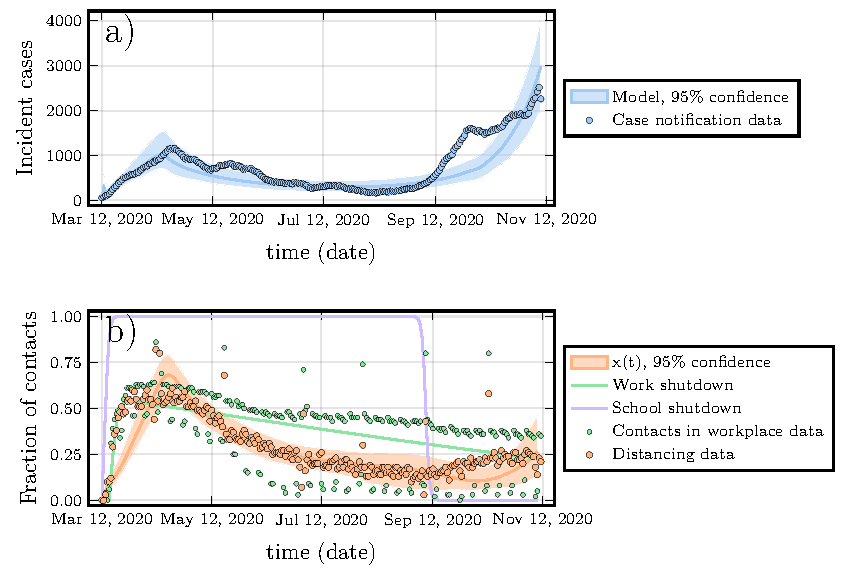
\includegraphics[width=\textwidth]{chapter_1/plot_model.pdf} 
\caption{A proxy for adherence to NPIs mirrors COVID-19 case reports in both data and model. (a) COVID-19 case incidence by date of report in Ontario, 7-day running average (circles) and ascertained case incidence from best fitting models (lines). (b) Percentage change from baseline in time spent at retail and recreation destinations (orange circles) and at workplaces (green circles) from Google mobility data, and proportion of the population $x$ adhering to NPIs (orange line) and workplace shutdown curve (green line) from fitted model.  Parameter values are provided in table \ref{tab:params}.}
\label{fig1}
\end{figure}

\begin{figure}
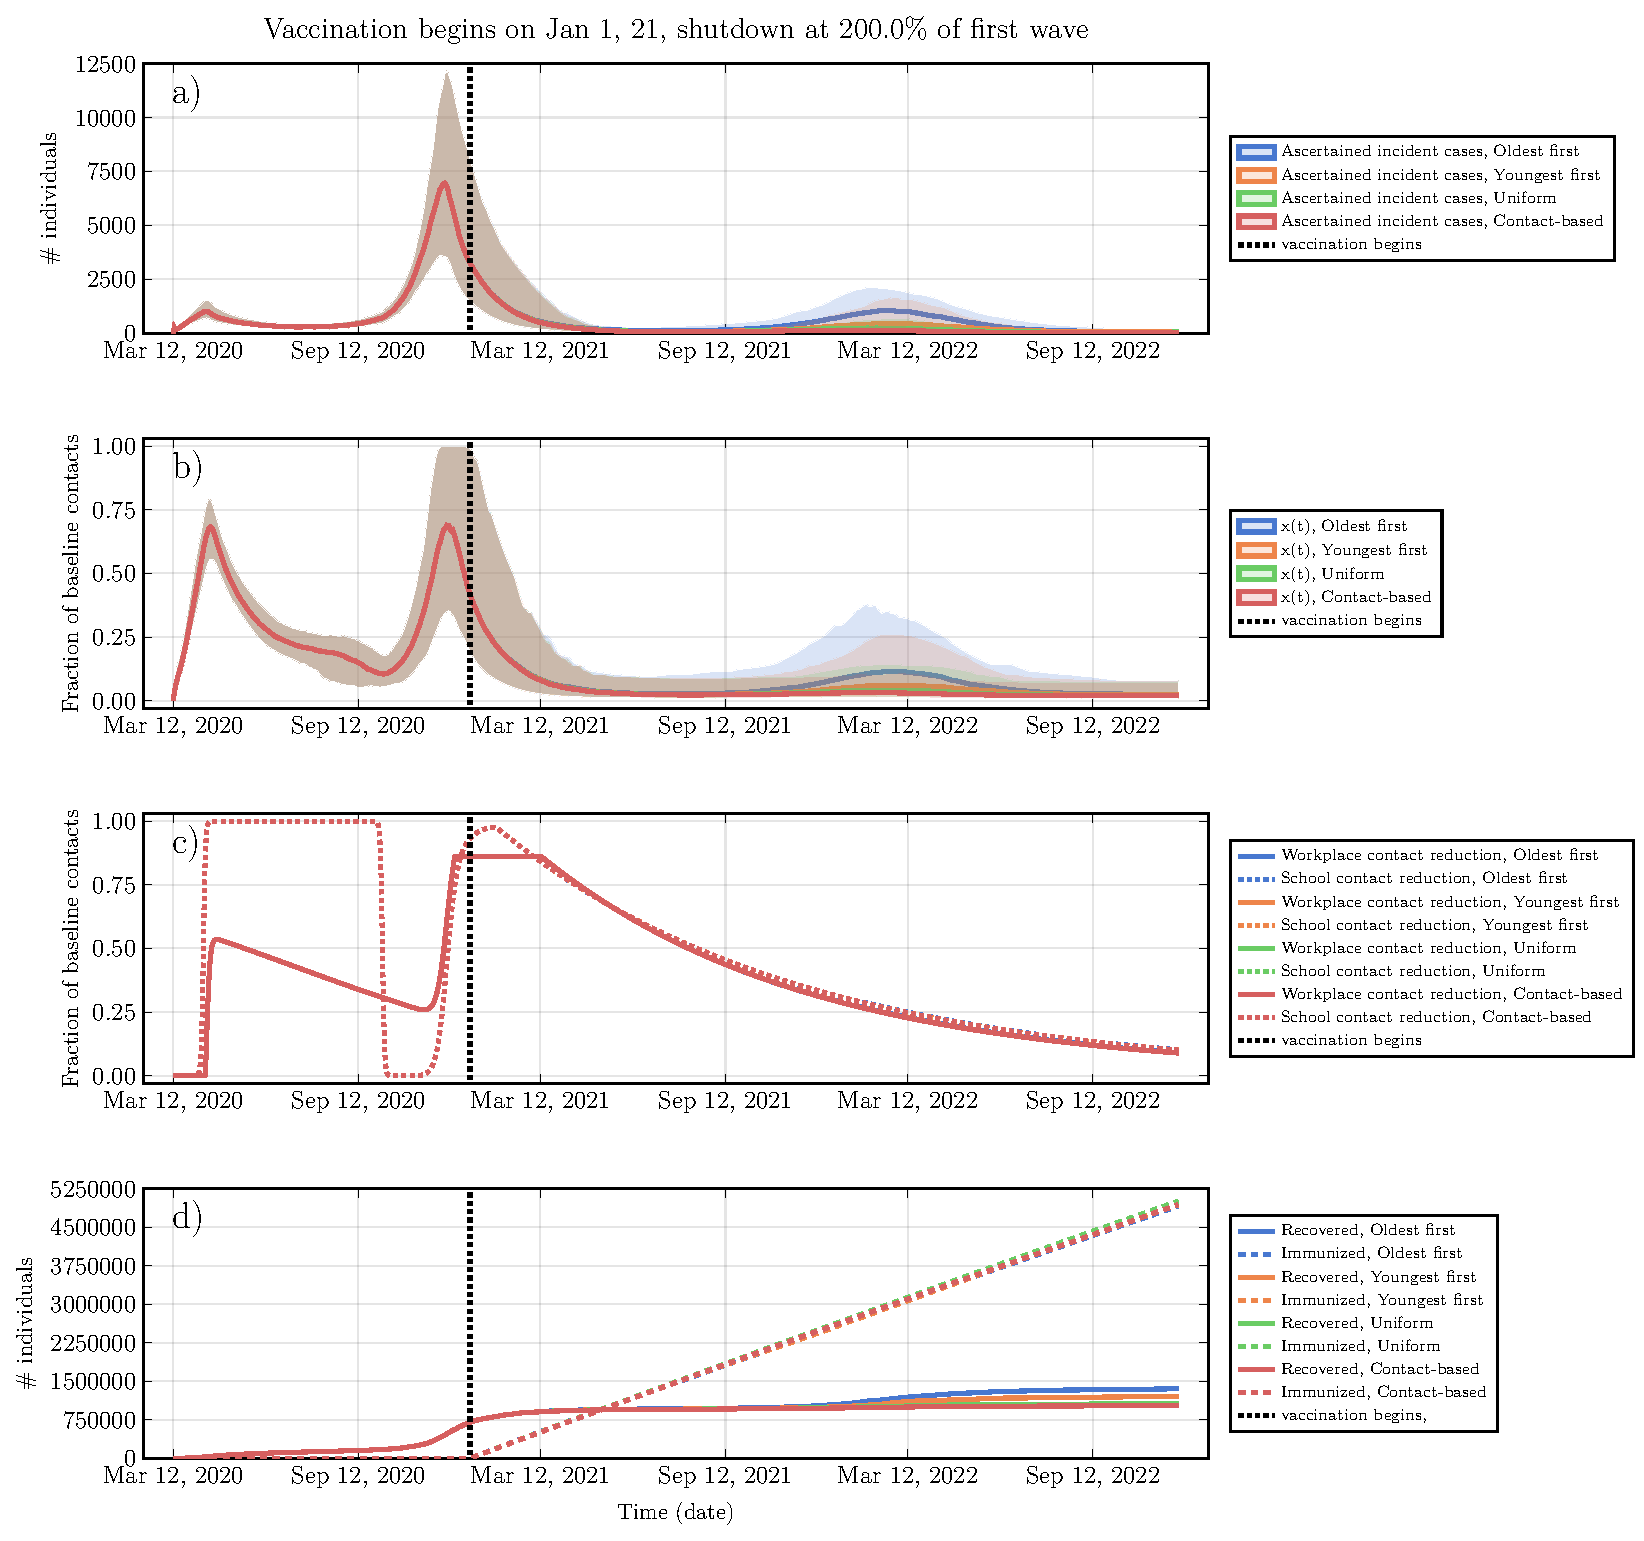
\includegraphics[width=\textwidth]{chapter_1/ts_plot.pdf}
\caption{Social and epidemiological dynamics interact to determine pandemic waves and vaccine strategy effectiveness. (a) Number of ascertained incident COVID-19 cases, (b) proportion $x$ of the population practicing NPIs, (c) level of school and workplace closure (note that curves for different vaccination strategies overlap), and (d) number of individuals with natural or vaccine-derived immunity versus time.  Ontario Population size: 14.6 million. Shutdown occurs at $T = 200$\% of peak cases in the first wave, vaccination starts in January 2021, vaccination rate is $\psi_0 =0.5\%$ per week. Other parameter values are provided in table \ref{tab:params}.}
\label{fig2}  
\end{figure}

\begin{figure}
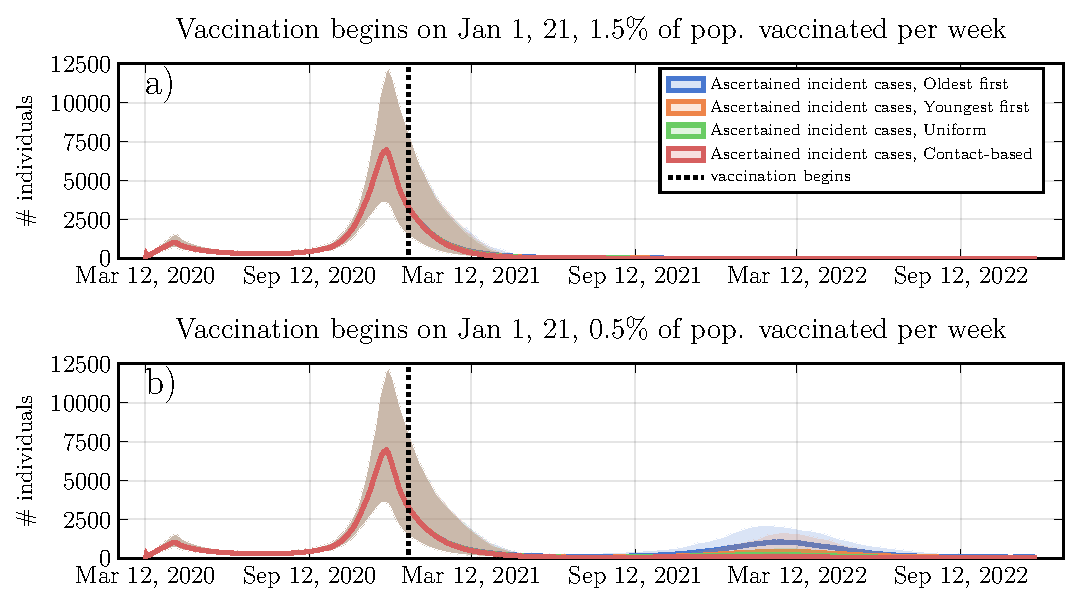
\includegraphics[width=\textwidth]{chapter_1/main_text_ts_1.pdf}
\caption{Three model regimes: (a) timely vaccination prevents third wave, (b,c) partial vaccination and indirect protection help during the third wave, and (d) slow and late vaccination fails to prevent third wave.  Projections of ascertained incident COVID-19 cases if vaccination begins in (a,b) January or (c,d) September, and if vaccinating (a,c) 1.5\% or (b,d) 0.5\% of the population per week. Ontario Population size: 14.6 million. $T = 200$\%. Other parameter values are provided in table \ref{tab:params}.}
\label{fig3}
\end{figure}


\begin{figure}
  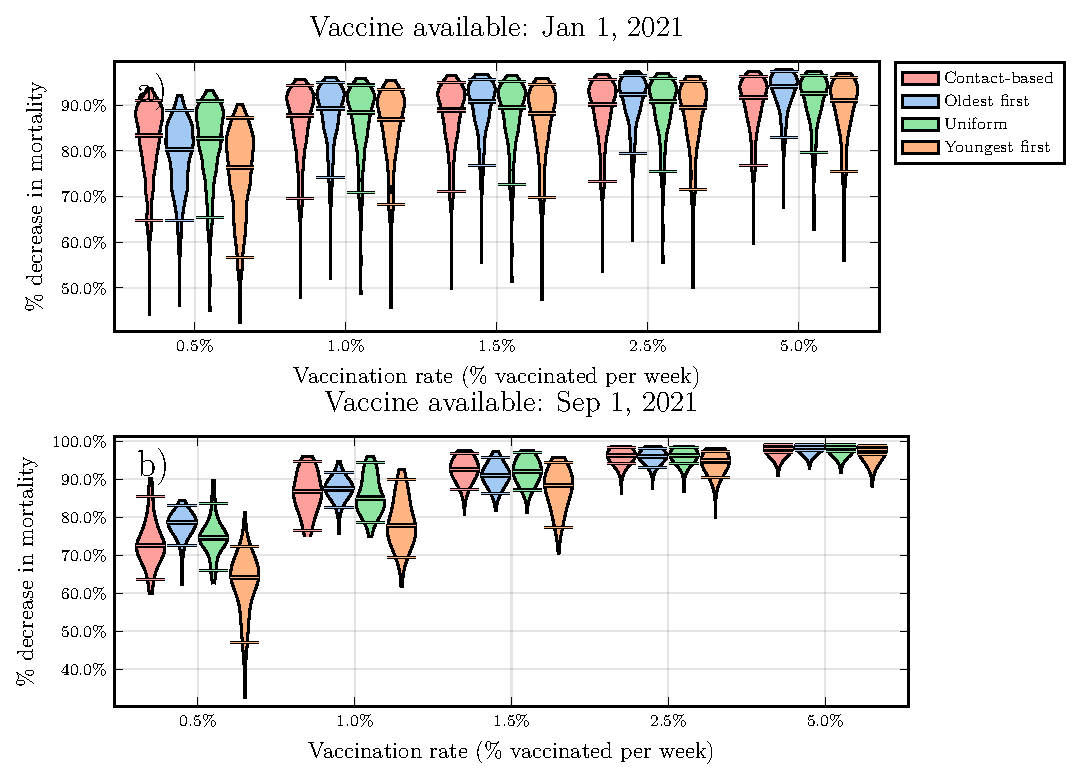
\includegraphics[width=\textwidth]{chapter_1/vaccination_by_mortality_small.pdf}  
  \caption{Percentage reduction in mortality for four strategies depends on vaccination start date and the vaccination rate.  Violin plots of the percent reduction in mortality under the four vaccine strategies, relative to no vaccination, as a function of the vaccination rate $\phi_0$, for (a) January and (b) September 2021 availability. Horizontal lines represent median values of posterior model projections. Shutdown threshold $T = 200\%$ and other parameter values are provided in table \ref{tab:params}. The projected number of deaths in the absence of vaccination was 72000 (95\% credible interval 40000–122000) from Jan 1, 2021, to March 14, 2025, and 60000 (31000–108000) from Sept 1, 2021, to March 14, 2025.}
  \label{fig4}
\end{figure}
\begin{figure}
  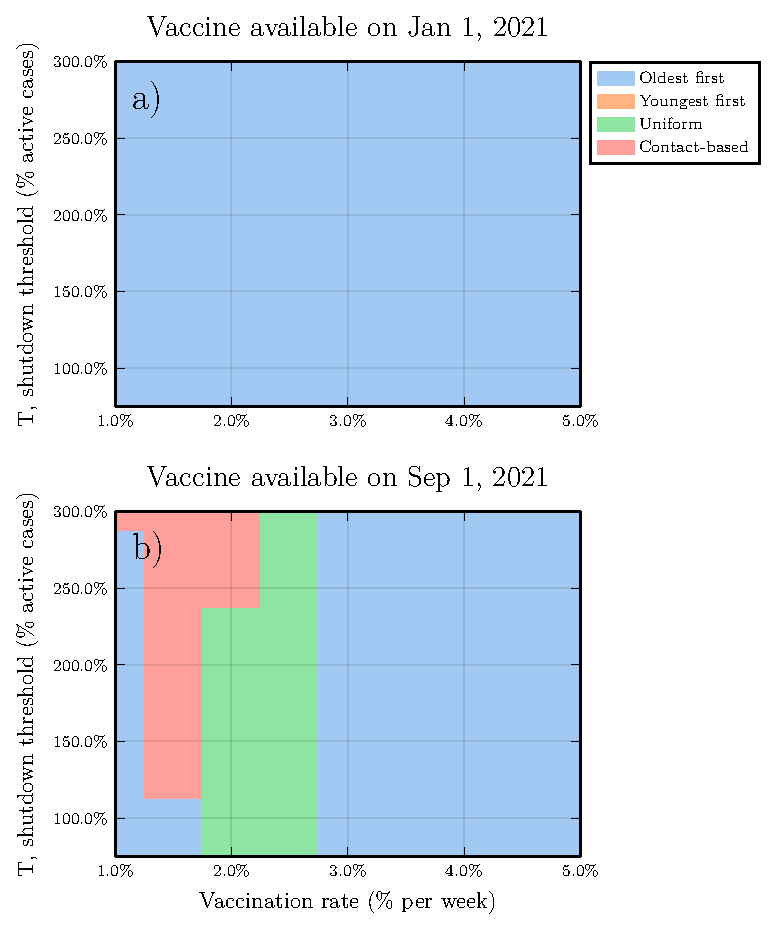
\includegraphics[width=\textwidth]{chapter_1/bivariate_heatmap.pdf}  
\captions{Best of four strategies depends on shutdown threshold T and vaccination rate $\phi_0$.  A later start to vaccination favours transmission-interrupting strategies for moderate vaccination rates.  Each parameter combination on the plane is colour coded according to which of the four strategies prevented the most deaths, on average across all model realizations, for (a) January and (b) September 2021 availability. Other parameter values are provided in table \ref{tab:params}.}
\label{fig5}
\end{figure}

\begin{figure}
  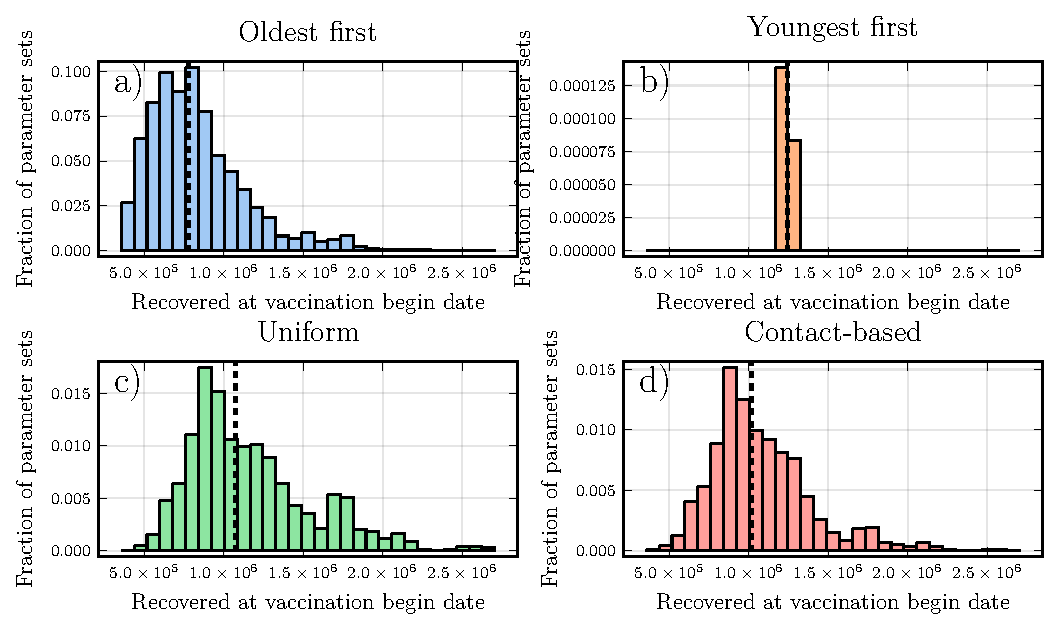
\includegraphics[width=\textwidth]{chapter_1/histograms.pdf}  
\caption{More pre-existing natural immunity makes transmission-interrupting strategies more effective. Frequency histogram of the percentage of the population with natural immunity for each strategy, taken from simulations where that strategy reduced mortality most effectively, for (a) oldest first, (b) youngest first, (c) uniform, and (d) contact-based strategies. The most effective strategy is defined as the one that reduced mortality the most across the largest number of model realizations. Vertical dashed lines denote median values of the distribution. Other parameter values are provided in table \ref{tab:params}.}
\label{fig6}
\end{figure}
The Google mobility data that we use as a proxy for adherence to NPIs closely mirrors the COVID-19 case notification data over the time period used for fitting (\ref{fig1}, open orange circles).  Since a heightened perception of COVID-19 infection risk simulates the adoption of NPIs26, which in turn reduces SARS-CoV-2 transmission \cite{anderson2020estimating,peak2020individual}, this exemplifies a coupled  social-epidemiological dynamic.  The mirroring may furthermore represent convergence between social and epidemiological dynamics, which has been predicted for strongly coupled systems \cite{sigdel2019convergence}. Moreover, the fit of the social submodel to the mobility data is as good as the fit of the epidemic submodel to case notification data (Figure \ref{fig1}), despite the fact that our social model consists of significantly fewer equations and a similar number of parameters as our epidemiological model. This shows how modelling population behaviour during a pandemic can be accomplished with relatively simple models. 

The model predicts additional pandemic waves from Fall 2020 onward, not only with respect to COVID-19 cases but also population adherence to NPIs and periods of school and workplace closure (Figure \ref{fig2}). The impact of the four strategies on COVID-19 cases and deaths depends on when the vaccine becomes available and how quickly the population can get vaccinated. Across a large parameter regime, vaccinating 60+ year-olds first prevents the most deaths out of all four strategies if vaccination begins in January 2021, whereas the uniform or contact-based strategies prevent the most deaths if vaccination begins in September 2021, unless the vaccination rate is very small or very large. More specifically, we identify three regimes for model dynamics. We explore them through plots of infection incidence over time (Figure \ref{fig3}); plots of the percentage reduction in mortality under all four strategies, as they depend on the vaccination rate (Figure \ref{fig4}) and shutdown threshold (Appendix, Figure \ref{s10}, \ref{s11}); and plots showing which of the four strategies prevents the most deaths as a function of the shutdown threshold and the vaccination rate (Figure \ref{fig5}). 

In the first regime, vaccination starts soon and the vaccination rate is relatively high (January availability, vaccinating 1.0\% or more of the population per week). A third wave in Fall 2021/Winter 2022 is thereby prevented (Figure \ref{fig3}a and Appendix, Figure \ref{s7}).  In this regime, enough people are vaccinated sufficiently far in advance to prevent a third wave, but the “oldest first” strategy prevents more deaths than the other strategies (Figure \ref{fig4}a, \ref{fig5}a). 

In the second regime, either vaccination starts early but the vaccination rate is too low (January availability, 0.5\% or less vaccinated per week, Figure \ref{fig2}, \ref{fig3}b, \ref{fig4}a), or vaccination starts late but the vaccination rate is high (September availability, vaccinating 1.5\% or more per week, Figure \ref{fig3}c, \ref{fig4}b and appendix, Appendix, Figure \ref{s8}).  In this intermediate scenario, a sufficient proportion of the population is vaccinated for indirect protection from the vaccine to become important during the third wave, but not enough individuals are vaccinated to completely prevent it.  As a result, the uniform and contact-based strategies are more effective than the 60+ first strategy, but the “youngest first” strategy does worst of all (Figure \ref{fig2}b, \ref{fig3}c, \ref{fig4}, \ref{fig5}).  The under-performance of the youngest first strategy occurs because in populations with strong age-assortative mixing26, the indirect benefits of vaccination are “wasted" if vaccination is first concentrated in specific age groups before being extended to the rest of the population.  The 60+ first strategy is less affected by this because the COVID-19 case fatality rate is high in this age group. However, as the vaccination rate becomes very high, the effectiveness of all four strategies converges, since the entire population is vaccinated quickly (Figure \ref{fig4}b).

In the third regime, vaccination starts late and the vaccination rate is low (September availability, 1.0\% or less vaccinated per week; Figure \ref{fig3}d and Appendix, Figure \ref{s9}). This scenario does not allow enough time for indirect protection from vaccination to become strong.  As a result, the oldest first strategy prevents more deaths than the other three strategies (Figure \ref{fig4}b, \ref{fig5}b).  Overall mortality is higher for all strategies, on account of the delayed rollout of the vaccine.  The relative performance of the strategies in these three regimes is generally unchanged across the full range of values for the shutdown threshold (Appendix, Figure \ref{s10}, \ref{s11}).  

Frequency histograms across all stochastic model realizations showing what percentage of the population has natural immunity at the start of a vaccine program, when a particular strategy was shown to work best, illustrate the role of indirect protection (Figure \ref{fig6}). In simulations where the “oldest first” strategy did best, the percentage of the population with natural immunity tends to be relatively low. This is expected, since indirect protection from vaccines is weaker when few people have natural immunity upon which vaccine indirect protection can build.  But when the uniform or contact-based strategy does best, more simulations exhibit a high level of natural immunity at the start of vaccination.  We note that the variance in these histograms is high, which underscores the role of other factors in the model such as timing and interaction between social and epidemiological dynamics. In a similar vein, if we plot the percentage reduction in mortality for hypothetical vaccination start dates ranging from September 2020 to September 2021, we observe that the transmission-interrupting strategies become relatively more effective than the “oldest first” strategy for later vaccination start dates, because herd immunity has time to increase before the start of the vaccine program (Appendix, Figure \ref{s12}). 

We also studied how the best strategy changes depending on vaccine efficacy ranging from 40-90\% in 60+ year-olds and in <60 year-olds (Appendix, Figure \ref{s13}).  For January vaccine availability, the “oldest first” strategy is best, even when vaccine efficacy is lower in 60+ year-olds than in those under 60 years of age.  For September vaccine availability, the uniform or contact-based strategies do best, except when vaccine efficacy in 60+ year-olds is higher than 70\% and also exceeds the vaccine efficacy in <60 year-olds. 

We modelled dynamics of vaccinating behaviour after vaccines become available (Appendix, Figures \ref{s14}, \ref{s15}, \ref{s16}).  Due to lack of empirical data, we explored a wide range for the social learning rate and the perceived relative cost of vaccination versus infection. The results suggest that a sufficiently high perceived cost of vaccination allows the uniform or contact-based strategies to outperform the “oldest first” strategy, especially for January vaccine availability, except when the vaccine social learning rate is also high (Appendix, Figure \ref{s14}). Vaccine refusal increases as the vaccine cost rises (Appendix, Figuresgs \ref{s14}, \ref{s15}, \ref{s16}). Since vaccine refusal in the targeted age group forces vaccination of other age groups instead, it makes all strategies behave more like the uniform strategy, although age-specific behaviours could change these predictions. 

We ran simulations with R0=2.5 for December 2020 onward and found that “oldest first” was more effective across a broader region of parameter space for September availability, particularly at higher vaccination rates (Appendix, Figure \ref{s18}). This is expected, since indirect protection is less effective when R0 is higher. We also ran simulations with 30\% higher and lower ascertainment for December 2020 onward to capture potential changes to COVID-19 testing and found that it had little impact on which strategy was most effective (Appendix, Figures \ref{s19}, \ref{s20}).  Similarly, higher or lower social learning rates for NPIs had little impact on the predictions (Appendix, Figures \ref{s21}, \ref{s22}). 

We also analyzed a scenario where the vaccine efficacy against disease can be greater than the vaccine efficacy against infectivity. We found that increasing the efficacy against disease up to 95\%, while holding the efficacy against infectivity constant at 75\%, caused a slight improvement in the effectiveness of all four strategies, especially for the “oldest first” and uniform strategies (Appendix, Figure \ref{s23}).  Finally, we generated results for our baseline scenario, but using a more stringent acceptance threshold for our Bayesian particle filtering algorithm. We found that our results were qualitatively unchanged (Appendix, Figure  \ref{s25}).  


\section{Discussion}

Our social-epidemiological model suggests that if a COVID-19 vaccine becomes available sufficiently late in the pandemic, using SARS-CoV-2 vaccines to interrupt transmission might prevent more COVID-19 deaths than using the vaccines to target those 60+ years of age, depending on when the vaccine becomes available and how quickly the population can be vaccinated. These results are driven by the fact that the vaccine may only become available after populations have had one or more waves of immunizing infections. As a result, the effective reproduction number $R_{eff}$ could be significantly closer to 1 than the basic reproduction number $R_0 \approx 2.2$ that applies to susceptible populations. In this regime, vaccines that reduce transmission have disproportionately large indirect protective effects \cite{anderson1992infectious}.

The Google mobility data that we use as a proxy for adherence to NPIs closely mirrors the COVID-19 case notification data over the time period used for fitting (Figure 1, open orange circles).  Since a heightened perception of COVID-19 infection risk simulates the adoption of NPIs \cite{wise2020changes}, which in turn reduces SARS-CoV-2 transmission \cite{anderson2020estimating, peak2020individual}, this exemplifies a coupled  social-epidemiological dynamic. This mirroring may represent convergence between social and epidemiological dynamics, which has been predicted for strongly coupled systems \cite{sigdel2019convergence}. Moreover, the fit of the social submodel to the mobility data is as good as the fit of the epidemic submodel to case notification data, despite the fact that our social model consists of significantly fewer equations and a similar number of parameters as our epidemiological model. This shows how modelling population behaviour during a pandemic can be accomplished with relatively simple models. 

Several studies have used compartmental models to study prioritisation of age groups for COVID-19 vaccination \cite{bubar2020model,hoyt2020vaccine,matrajt2020vaccine}. These models vary widely in terms of study populations, representation of population heterogeneity, interventions, and assumptions about when vaccination starts. Similar to our results, Matrajt et al \cite{matrajt2020vaccine}  find that the level of pre-existing immunity strongly dictates outcomes: when pre-existing immunity is high, strategies that distribute the vaccine more evenly across age groups rather than prioritising older age groups. Buckner et al \cite{hoyt2020vaccine} find that targeting 60+ year-olds is best for reducing mortality. They assumed that vaccination begins in December 2020, and they base initial conditions on case notifications in the United States in that month. Similarly, Bubar et al \cite{bubar2020model} find that vaccinating 60+ year-olds works best for reducing mortality for vaccine programs starting in July 2020 in Belgium, or August 2020 in New York City. Our results agree with Refs. \cite{bubar2020model,hoyt2020vaccine} for the scenario of January 2021 vaccine availability. However, we find more deaths can be prevented by first vaccinating other age groups for a September 2021 start. Such a late vaccine start date was not analyzed in \cite{bubar2020model,hoyt2020vaccine} although their findings might change if the models were re-initialized to accommodate vaccination starting in September 2021. 

Our analysis was limited by its focus on prioritisation of age groups. We did not model other sources of heterogeneity such as geography, socio-economic status, sex, or race--all of which are important determinants of disease burden in this highly unequal pandemic. We did not model outbreaks in long-term care facilities, where the dynamics of transmission and indirect protection differ from the general population. Similarly, we did not distinguish healthcare or other essential workers. However, many of these individuals are working age adults, and thus vaccinating them first among other working adults is consistent with our uniform and contact-based strategies.  For our baseline analysis we assumed the vaccine blocks transmission as well as it prevents COVID-19 disease. But in general, vaccines have differing efficacy in this regard \cite{hodgson2020defines}. This can reduce the relative benefits of strategies intended to interrupt transmission.  We used a single population model, but inter-population mobility can influence transmission dynamics: a large influx of infectious persons from another population can weaken the indirect protection afforded by vaccines. 

We used changes to baseline time spent at retail and recreational outlets to represent population adherence to NPIs.  Such mobility data is an imperfect proxy for physical distancing and will not capture mask use or hand-washing.  We did not have high resolution mobility data on these practices, although in future it may be possible to infer information about these practices by combining information from phone surveys with online social media data. Our simple ascertainment process in the model was designed to implicitly capture the effects of COVID-19 PCR testing, contact tracing and isolation (TTI). But without explicitly representing them, it is impossible for us to study combined strategies of vaccination and TTI, or to anticipate how specific changes to TTI would influence our findings. 

Finally, the model was parameterised with data from Ontario, Canada. For instance, the emergence of a more transmissible strain of SARS-CoV-2 would weaken the indirect protection provided by a vaccine that reduces transmission. At the same time, we note that our findings rely upon a robust epidemiological effect that occurs when $R_eff$ becomes sufficiently small. Therefore, the only thing that may change in other settings is the timing of the switch to vaccine strategies that interrupt transmission. 


We opted for a coupled social-epidemiological model on account of the importance of interactions between population behaviour and disease dynamics for the control of COVID-19 in the absence of preventive pharmaceutical interventions. Our model generated significantly different projections in our sensitivity analysis where population behaviour was assumed constant, which is similar to conventional approaches to transmission modelling. Our social model is less complicated than our epidemiological model and despite this, the coupled social-epidemiological model fitted population-level behaviour as readily as it fitted the epidemic curve. Predicting behaviour is fraught with uncertainty, but so is predicting an epidemic curve. Moreover, digital data on behaviour and sentiment that can be used to model social dynamics is increasingly available \cite{salathe2012digital}.  Given this, we suggest a role for more widespread use of  social-epidemiological models during pandemics. 

To apply these results to COVID-19 pandemic mitigation, large-scale seroprevalence surveys before the onset of vaccination could ascertain the level of a population's natural immunity.  Age-structured compartmental models could be initialized with this information to generate population-specific projections. In populations where SARS-CoV-2 seropositivity is high due to a Fall/Winter 2020 wave, vaccinating to interrupt transmission may reduce COVID-19 mortality more effectively than targeting vulnerable groups. 

